% paper.tex
%
% LaTeX template for creating an MNRAS paper
%
% v3.0 released 14 May 2015
% (version numbers match those of mnras.cls)
%
% Copyright (C) Royal Astronomical Society 2015
% Authors:
% Keith T. Smith (Royal Astronomical Society)

% Change log
%
% v3.0 May 2015
%    Renamed to match the new package name
%    Version number matches mnras.cls
%    A few minor tweaks to wording
% v1.0 September 2013
%    Beta testing only - never publicly released
%    First version: a simple (ish) template for creating an MNRAS paper

%%%%%%%%%%%%%%%%%%%%%%%%%%%%%%%%%%%%%%%%%%%%%%%%%%
% Basic setup. Most papers should leave these options alone.
\documentclass[a4paper,fleqn,usenatbib]{mnras}

% MNRAS is set in Times font. If you don't have this installed (most LaTeX
% installations will be fine) or prefer the old Computer Modern fonts, comment
% out the following line
\usepackage{newtxtext,newtxmath}
% Depending on your LaTeX fonts installation, you might get better results with 
% one of these:
%\usepackage{mathptmx}
%\usepackage{txfonts}

% Use vector fonts, so it zooms properly in on-screen viewing software
% Don't change these lines unless you know what you are doing
\usepackage[T1]{fontenc}
\usepackage{ae,aecompl}


%%%%% AUTHORS - PLACE YOUR OWN PACKAGES HERE %%%%%

% Only include extra packages if you really need them. Common packages are:
\usepackage{graphicx}	% Including figure files
\usepackage{amsmath}	% Advanced maths commands
\usepackage{amssymb}	% Extra maths symbols
\usepackage{mathtools}

%%%%%%%%%%%%%%%%%%%%%%%%%%%%%%%%%%%%%%%%%%%%%%%%%%

%%%%% AUTHORS - PLACE YOUR OWN COMMANDS HERE %%%%%

\newcommand{\fesc}{\ifmmode{f_{\rm esc}}\else{$f_{\rm esc}$}\fi}
\newcommand{\fescs}{\ifmmode{f_{\rm esc}^\star}\else{$f_{\rm esc}^\star$}\fi}
\newcommand{\kms}{\ifmmode{{\;\rm km~s^{-1}}}\else{km~s$^{-1}$}\fi}
\newcommand{\fgas}{\ifmmode{{f_{\rm gas}}}\else{$f_{\rm gas}$}\fi}
\newcommand{\cubecm}{\ifmmode{{\rm cm^{-3}}}\else{cm$^{-3}$}\fi}
\newcommand{\ztwo}{\ifmmode{{\rm [Z_2/H]}}\else{[Z$_2$/H]}\fi}
\newcommand{\zthree}{\ifmmode{{\rm [Z_3/H]}}\else{[Z$_3$/H]}\fi}
\newcommand{\lsim}{\lower0.3em\hbox{$\,\buildrel <\over\sim\,$}}
\newcommand{\gsim}{\lower0.3em\hbox{$\,\buildrel >\over\sim\,$}}
\newcommand{\li}{\noindent$\bullet$\quad}
\newcommand{\lli}{$\bullet$\quad}
\newcommand{\lcdm}{$\Lambda$CDM}
\newcommand{\flux}{erg s$^{-1}$ cm$^{-2}$ Hz$^{-1}$}
\newcommand{\emis}{erg s$^{-1}$ cm$^{-2}$ Hz$^{-1}$ sr$^{-1}$}
\newcommand{\sfr}{\ifmmode{\textrm{M}_\odot \,\textrm{yr}^{-1} \,\textrm{Mpc}^{-3}}\else{M$_\odot$ yr$^{-1}$ Mpc$^{-3}$}\fi}
\newcommand{\hsfr}{\ifmmode{\textrm{M}_\odot\, \textrm{yr}^{-1}}\else{M$_\odot$ yr$^{-1}$}\fi}
\newcommand{\ssfr}{Gyr$^{-1}$}
\newcommand{\arp}{$a_{\rm rp}$}
\newcommand{\agrav}{$a_{\rm grav}$}
\newcommand{\eavg}{\ifmmode{\langle E_\gamma \rangle}\else{$\langle E_\gamma \rangle$}\fi}
\newcommand{\hst}{{\it HST}}
\newcommand{\enzo}{{\sc enzo}}
\newcommand{\yt}{{\sc yt}}
\newcommand{\moray}{{\sc enzo+moray}}
\newcommand{\Ms}{\ifmmode{M_\odot}\else{$M_\odot$}\fi}
\newcommand{\vrms}{\ifmmode{v_{\rm rms}}\else{$v_{\rm rms}$}\fi}
\newcommand{\mmin}{M$_{min}$}
\newcommand{\hh}{H$_2$}
\newcommand{\Ol}{$\Omega_\Lambda$}
\newcommand{\Om}{$\Omega_M$}
\newcommand{\Ob}{$\Omega_b$}
\newcommand{\theat}{$t_{\rm{heat}}$}
\newcommand{\tcool}{$t_{\rm{cool}}$}
\newcommand{\rcool}{$r_{\rm{cool}}$}
\newcommand{\tcross}{$t_{\rm{cross}}$}
\newcommand{\tdyn}{$t_{\rm{dyn}}$}
\newcommand{\tkh}{$t_{\rm{KH}}$}
\newcommand{\tH}{$t_{\rm{H}}$}
\newcommand{\tvir}{\ifmmode{T_{\rm{vir}}}\else{$T_{\rm{vir}}$}\fi}
\newcommand{\mvir}{\ifmmode{M_{\rm{vir}}}\else{$M_{\rm{vir}}$}\fi}
\newcommand{\rvir}{\ifmmode{r_{\rm{vir}}}\else{$r_{\rm{vir}}$}\fi}
\newcommand{\rr}{$r_{200}$}
\newcommand{\lya}{Ly$\alpha$}
\newcommand{\jj}{\ifmmode{J_{21}}\else{$J_{21}$}\fi}
\newcommand{\flw}{\ifmmode{F_{LW}}\else{$F_{LW}$}\fi}
\newcommand{\kph}{\ifmmode{k_{\rm ph}}\else{$k_{\rm ph}$}\fi}
\newcommand{\tv}{$\langle T \rangle_{\rm v}$}
\newcommand{\tm}{$\langle T \rangle_{\rm m}$}
\newcommand{\msun}{{\rm\,M_\odot}} 
\newcommand{\lsun}{{\rm\,L_\odot}}
\newcommand{\zsun}{\ifmmode{\rm\,Z_\odot}\else{$\rm\,Z_\odot$}\fi}
\newcommand{\etal}{et al.\ }
\newcommand\tento[1]{$10^{#1}$}
\newcommand\step[1]{\textit{Step #1}.--}
\newcommand\halo[1]{\textit{Halo #1}.--}
\newcommand{\hi}{H {\sc i}}
\newcommand{\hii}{H {\sc ii}}
\newcommand{\hei}{He {\sc i}}
\newcommand{\heii}{He {\sc ii}}
\newcommand{\heiii}{He {\sc iii}}
\newcommand{\nhi}{\ifmmode{N_{\rm HI}}\else{$N_{\rm HI}$}\fi}
\newcommand\unit[1]{\; \textrm{#1}}
\newcommand{\pem}{\unit{s}^{-1} \unit{cMpc}^{-3}}
\newcommand{\music}{{\sc Music}}
\newcommand{\rockstar}{{\sc Rockstar}}

\newcommand{\refs}{(\textbf{Add references})}
\newcommand{\jhw}[1]{{\color{red} \bf (JHW: #1)}}


%%%%%%%%%%%%%%%%%%%%%%%%%%%%%%%%%%%%%%%%%%%%%%%%%%
%% Additions from AASTeX
%%%%%%%%%%%%%%%%%%%%%%%%%%%%%%%%%%%%%%%%%%%%%%%%%%

%\newcommand\ion[2]{#1$\;${\small\rmfamily\@Roman{#2}}\relax}
\def\eps@scaling{1.0}% 
\newcommand\epsscale[1]{\gdef\eps@scaling{#1}}% 
\newcommand\plotone[1]{% 
 \centering 
 \leavevmode 
 \includegraphics[width={\eps@scaling\columnwidth}]{#1}% 
}% 
\newcommand\plottwo[2]{% 
 \centering 
 %\leavevmode 
 %\columnwidth=.5\columnwidth 
 \includegraphics[width={\eps@scaling\columnwidth}]{#1}% 
 \hfil 
 \includegraphics[width={\eps@scaling\columnwidth}]{#2}% 
}% 

% \newcommand{\nat}{Nature}
% \newcommand{\aj}{AJ}
% \newcommand{\apj}{ApJ}
% \newcommand{\apjl}{ApJL}
% \newcommand{\apjs}{ApJS}
% \newcommand{\mnras}{MNRAS}
% \newcommand{\aap}{A\&A}
% \newcommand{\pasj}{PASJ}
% \newcommand{\pasp}{PASP}
% \newcommand{\araa}{ARA\&A}
% \newcommand{\bain}{Bull.~Astron.~Inst.~Netherlands}
% \newcommand{\memsai}{Mem.~Soc.~Astron.~Italiana}
% \newcommand{\physrep}{Physics Reports}
% \newcommand{\prd}{Phys.~Rev.~D}
% \newcommand{\jcap}{JCAP}

\hyphenation{sSFR sSFRs}

\makeatletter
\newcommand*{\rom}[1]{\expandafter\@slowromancap\romannumeral #1@}
\makeatother

% Please keep new commands to a minimum, and use \newcommand not \def to avoid
% overwriting existing commands. Example:
%\newcommand{\pcm}{\,cm$^{-2}$}	% per cm-squared

%%%%%%%%%%%%%%%%%%%%%%%%%%%%%%%%%%%%%%%%%%%%%%%%%%

%%%%%%%%%%%%%%%%%%% TITLE PAGE %%%%%%%%%%%%%%%%%%%

% Title of the paper, and the short title which is used in the headers.
% Keep the title short and informative.
\title[Where Do Pop III Stars Form?]{Where Do Population III Stars Form?}

% The list of authors, and the short list which is used in the headers.
% If you need two or more lines of authors, add an extra line using \newauthor
\author[Danielle Skinner et al.]{
Danielle Skinner,$^{1}$\thanks{E-mail: drenniks@gatech.edu}
John H. Wise,$^{1}$
\\
% List of institutions
$^{1}$Center for Relativistic Astrophysics, Georgia Institute of Technology, 
Atlanta, GA 30332, USA\\
}

% These dates will be filled out by the publisher
%\date{Accepted XXX. Received YYY; in original form ZZZ}

% Enter the current year, for the copyright statements etc.
\pubyear{2018}

% Don't change these lines
\begin{document}
\label{firstpage}
\pagerange{\pageref{firstpage}--\pageref{lastpage}}
\maketitle

% Abstract of the paper
\begin{abstract}
This is a simple template for authors to write new MNRAS papers.
The abstract should briefly describe the aims, methods, and main results of the 
paper.
It should be a single paragraph not more than 250 words (200 words for Letters).
No references should appear in the abstract.
\end{abstract}

% Select between one and six entries from the list of approved keywords.
% Don't make up new ones.
\begin{keywords}
keyword1 -- keyword2 -- keyword3
\end{keywords}

%%%%%%%%%%%%%%%%%%%%%%%%%%%%%%%%%%%%%%%%%%%%%%%%%%

%%%%%%%%%%%%%%%%% BODY OF PAPER %%%%%%%%%%%%%%%%%%
%====================================================================
\section{Introduction}
%====================================================================

The first generation of stars transformed a cold and dark universe
by illuminating and enriching up their neighborhoods with radiation
and heavy elements. The formation of these first stars is a crucial step in the cosmological evolution of the universe because the metals and feedback they deliver to their local environments is necessary for further star production and chemical enrichment. Without these initial stars, heavier metals would not have been produced, and a different universe would be observed than what is observed today. These stars are, by definition, metal-free (Population III; Pop III) and are thought to be generally massive. A substantial fraction of these stars will generate prodigious amounts of ionizing photons and will end their lives in some form of a supernova \citep[e.g.][]{Schaerer02, Heger02}. The supernova will spread the enriched guts of the Pop III star out across its local environment, providing the area with elements the universe has not yet seen. 

Once a halo becomes chemically enriched by the death of its Pop III stars, then by definition, it can no longer form more Pop III stars. This marks the end of metal-free star formation in that pregalactic object. Understanding the mixing of metals into the environment of these halos is necessary to constrain the reach of these metals and the effects they have for future star formation. Numerical studies have shown that turbulence within halos can mix metals well down to their resolution limit \citep[][and more]{Wise08_Gal, Greif10}. Stars will continue to form in halos, but with an increased metal abundance, these stars are now labelled as metal-enriched stars. These stars still are considered metal-poor, relative to the solar abundance, and are observable in the universe. Understanding the formation and chemical abundance of second generation stars can provide more evidence and insight for the earlier generation of Pop III stars.

Given the paradigm of hierarchical structure formation, halos grow through smooth accretion and successive mergers of smaller halos. But in which halos do these first generations of stars form? Their formation rates and locations are important to constrain because they influence the very beginnings of galaxy formation and cosmic reionization. Learning about their host halos can also guide future telescopic surveys to observe Pop III galaxies which may lead to direct observational evidence for Pop III stars. Previous studies have investigated the possibility of finding Pop III systems. \citet{Trenti09} found that metal-free halos may still be able to form at $z \approx$ 6, which offer the best chance at observing such primordial systems. Given a certain rate of Pop III supernova per year, large sky surveys, such as the Large Synoptic Survey Telescope (LSST), should be able to detect the very luminous supernova. Unless the metal-free systems are particularly efficient at forming Pop III stars (star formation efficiences > 10$^{-2}$), the upcoming James Webb Space Telescope (JWST) will not be able to detect such systems.

Various semi-analytic investigations have been conducted to learn more about the halo collapse criterion, and thus, which halos can host Pop III stars. \citet{Tegmark97} discovered that halos can have a strongly redshift dependent, minimum baryonic mass of 10$^{6}$ M$_{\odot}$ at $z \approx$ 15. In particular, they derive an analytic expression for the fraction of \hh{} needed in a halo for efficient cooling, and determine which  halos can cool in a Hubble time. \citet{Visbal18} came up with a semi-analytic model for the formation of Pop III stars and the transition from Pop III to metal-enriched stars. They find that varying the Pop III star formation efficiency, the time from a Pop III supernova to metal-enriched star formation, the external enrichment of the halo, and the ionizing espcape fraction, leads to large differencies in the star formation history of Pop III and metal-enriched stars. This method is useful for exploring the wide parameter space of star formation in the early universe, and could lead to further constraints in the future. 

Without metals and dust to facilitate efficient radiative cooling, Pop III stars rely on \hh{} formation to cool the gas. These molecules are however fragile to dissociation from Lyman-Werner (LW) radiation in the energy range 11.2--13.6~eV, through the Solomon process \citep{Field66, Stecher67}. This is a two-step process through which H$_{2}$ is excited to a higher state, H$_{2}^{\ast}$, via absorption of a LW photon:
\begin{equation} \label{Solomon1}
	H_{2} + \gamma \rightarrow  H_{2}^{\ast}
\end{equation}
This excited state then has a probability of dissociating into two hydrogen atoms:
\begin{equation} \label{Solomon2}
	H_{2}^{\ast} \rightarrow H + H
\end{equation}

Diffuse gas is optically thin to LW radiation, thus a background builds over time and can suppress \hh{} formation, prohibiting Pop III star formation. Furthermore, nearby sources of LW radiation can boost the intensity above the background value which facilitates further \hh{} dissociation in minihalos. This process can be counteracted with a sufficient amount of \hh{} already present within a halo, via \hh{} self-shielding. Halos with an \hh{} column density of N$_{H_{2}}$ $\geq$ 10$^{14}$ cm$^{-2}$ can suppress the photodissociation of \hh{} by LW photons, giving the halo a chance to form Pop III stars. Other sources of the suppression of Pop III star formation are streaming baryonic velocities, arising from recombination, and dynamical heating, occuring during the virialization of halos. 

Previous work have mainly investigated and established the lower limit for a halo to host Pop III stars, or for a halo to collapse. However, subsequent simulations have shown that they do not necessarily form at this minimum due to the aforementioned physical processes playing a role. \citet{Mebane18} used a semi-analytic model of early star formation and found that the LW background coming from the rapidly increasing supply of Pop III stars becomes responsible for suppressing Pop III star formation. Pop III supernova feedback is another key process which can allow Pop III stars to continue to form, as long as the metals are ejected from the host halo. \citet{Griffen18} also find that the LW background can significantly suppress the amount of potential sites for Pop III star formation. 

Numerical simulations have also been employed to investigate collapse thresholds and Pop III star formation. \citet{Machacek01} found similar results to those mentioned previously, in that the LW feedback can suppress the collapse of small mass halos. They derive a simple analytic expression for the mass threshold of halos given a particular LW flux. We will compare our results with this relation in future sections. \citet{Yoshida03} also finds that cooling is inefficient in halos with a LW background > 0.01, although with sufficient \hh{} shielding, halos are able cool in the given LW background radiation. In fact, \citet{Wise07_UVB} found that central shocks drive \hh{} formation, allowing the halo to cool in a LW background flux of 10$^{-20}$. They find that \hh{} cooling is always a dominant process, even in large LW background fluxes. Assisting this result, \citet{OShea08} find that Pop III star formation can occur in relatively high LW backgrounds, implying that the LW background may not be a complete indicator of whether or not Pop III stars will form in a given halo.  

In this paper, we focus on the distribution of host halo masses, not just the minimum, and its dependence on redshift and the LW background, augmenting results from prior work. We aim to provide further insight into the host halos of Pop III stars. In \S 2 the methods of the simulation, implementation of star formation, feedback, and \hh{} self-shielding is described. In \S 3 we present the results of our analysis. In \S 4 we discuss the results in more detail and compare with previous work. In \S 5 we conclude our discussion with a summary of our results and the implications therein.

%====================================================================
\section{Methods}
%====================================================================
\subsection{Simulation setup}
%====================================================================
This simulation was run with an adaptive mesh refinement (AMR) code 
\enzo{} \citep{Enzo} and analyzed with the toolkit, \yt{} \citep{yt_full_paper}. \enzo{} uses an N-body adaptive particle-mesh solver \citep{Efstathiou85, Couchman91, BryanNorman1997} to follow the dark matter (DM) dynamics. We use the nine-species (\hi, \hii, \hei, \heii, \heiii, e$^{-}$, H$_{2}$, H$_{2}^{+}$, H$^{-}$) non-equilibrium chemistry model \citep{Abel97, Anninos97}. This simulation is similar to the RP simulation in 
\citet[hereafter W12]{Wise12_RP}, but with updated cosmological and Pop III parameters, and the inclusion of \hh{} shielding.

We simulate a 1 Mpc$^{3}$ comoving box with a 256$^{3}$ base grid 
resolution. We have a maximum refinement level of 12 which provides a maximal comoving resolution of $\sim$1 pc. The simulation is 
initialized with \music{} \citep{Hahn11_MUSIC} at $z$ = 130 and use the cosmological parameters from the Planck collaboration best fit 
\citet{Planck13_Cosmo}: $\Omega_{M}$ = 0.3175, $\Omega_{\Lambda}$ = 
0.6825, $\Omega_{DM}$ = 0.2685, and h = 0.6711, with the variables 
having their usual definitions. The simulation is run until $z$ = 9.32, when it becomes too computationally expensive to continue. At this point, 20\% of the volume is ionized. In this paper, we focus only on outputs where new Pop III stars are born, from $z$ = 27.23 to 9.39. 

A time-dependent LW optically thin radiation background is applied in the simulation. This was fit in W12 (see their Eq. 16) and is consistent with the values in \citet{Trenti09_SFR}. The background evolution of the specific intensity takes the following form:
\begin{equation} \label{LWbg}
	\log_{10}(J_{LW}/J_{21}) = A + Bz - Cz^{2} + Dz^{3} - Ez^{4}
\end{equation}
where $(A, B, C, D, E)$ = $(-2.567, 0.4562, - 0.02680, 5.882 \times 10^{-4}, - 5.056 \times 10^{-6})$ and J$_{21}$ is a specific intensity of 10$^{-21}$ erg s$^{-1}$ cm$^{-2}$ Hz$^{-1}$ sr$^{-1}$. 

Adaptive ray tracing \citep{Abel02_RT, Wise11_Moray} is used to evolve the radiation field. Centered on each metal-enriched and Pop III star, we model the \hh{} dissociating radiation field with an optically thin, inverse square profile. These LW sources are added on top of the background intensity described above.
%====================================================================
\subsection{Star formation}
%====================================================================
In this section, we will discuss how we implement Pop III and metal-enriched star formation. We do not consider the formation and feedback from stellar remnants or asymptotic giant branch (AGB) stars. For further details, we refer the reader to W12. 

%====================================================================
\subsubsection{Pop III Star Formation and Feedback }
%====================================================================
The implemented Pop III star formation model is the same as in Wise \& Abel (2008). Each star particle represents a single star, and is formed in a cell when the following criteria are met: 
\begin{enumerate}
	\item a metallicity Z $\leq$ 5 $\times$ 10$^{-6}$ Z$_{\odot}$

	\item a gas number density n > 10$^{6}$ cm$^{-3}$

	\item converging gas flow, $\nabla \cdot \mathbf{v_{gas}}$ < 0 

	\item molecular hydrogen fraction, f$_{\rm H2}$ > 10$^{-3}$
\end{enumerate}

If within 1 pc, multiple cells meet this criteria, then a single Pop III star forms at the center of mass of these cells. The mass of the Pop III star is randomly sampled from an initial mass function (IMF) of the form:
\begin{equation} \label{IMF}
	f(\log M)dM = M^{-1.3} \exp \Big[-\left( \frac{M_{\rm char}}{M}\right)^{1.6} \Big]dM
\end{equation}
where M$_{\rm char}$ = 20 M$_{\odot}$. This characteristic mass is different from W12 and W14 (would like to find a citation for this number, having a hard time tracking down some John had suggested). This results in an exponential cutoff before M$_{char}$ and a Salpeter IMF after. Once the cell meets the above criteria and the mass of the star is randomly determined from Eq. 3, an equal amount of gas is removed from the grid in a sphere which contains twice the stellar mass that is centered on the new star particle. The new Pop III star then gains the mass-weighted velocity of the gas contained within that sphere.  

We use the mass-dependent hydrogen ionising LW luminosities and lifetimes from \citet{Schaerer02} and a mass-independent photon energy of E$_{ph}$ = 29.6 eV, which is appropriate for the nearly mass-independent surface temperature of Pop III stars, at 10$^{5}$ K. A Type II supernova results if the Pop III star dies with a mass between 11 $\leq$ M$_{\ast}$/M$_{\odot}$ $\leq$ 40 M$_{\odot}$. A pair instability supernova (PISNe) results if the star dies with a mass between 140 $\leq$ M$_{\star}$/M$_{\odot}$ $\leq$ 260 M$_{\odot}$. Outside of these mass ranges, the Pop III star dies as a black hole. In this simulation, no black hole physics are implemented, so the Pop III star simply turns into a collisionless particle. From 11 $\leq$ M$_{\star}$/M$_{\odot}$ < 20 M$_{\odot}$, the star dies as a normal Type II supernova with an energy of 10$^{51}$ erg. From 20 $\leq$ M$_{\star}$/M$_{\odot}$ $\leq$ 40 M$_{\odot}$, the star dies as a hypernova with energies taken from \citet{Nomoto06}.The PISNe have explosion energies from \citet{2002ApJ...567..532H}, of which the analytic function fit to their models can be seen in Eq. 12 of W12. 

%====================================================================
\subsubsection{Pop II  Star Formation and Feedback}
%====================================================================
The Pop II star formation model is the same as Wise \& Cen (2009), which is equivalent to the above criteria for Pop III star formation but without the molecular hydrogen fraction requirement, and with a metallicity greater than the above value. Star formation is only allowed for gas with temperatures $T$ < 1000 K, to ensure that the volume is cold and collapsing. Contrary to Pop III stars representing single star particles, metal-enriched star particles are modelled as clusters of stars. We enforce a minimum mass of M$_{min}$ = 1000 M$_{\odot}$ for these star particles. 

The lifetime of these particles is 20 Myr, during which they radiate 6000 hydrogen ionising photons per stellar baryon, or 1.13 $\times$ 10$^{46}$ photons s$^{-1}$ M$_{\odot}^{-1}$, which is appropriate for a Salpeter IMF. Their spectra are approximated with a monochromatic spectrum with an energy of 21.6 eV at a constant luminosity. After living for 4 Myr, the stars generate supernova energies of 6.8 $\times$ 10$^{48}$ erg s$^{-1}$ M$_{\odot}^{-1}$.

%====================================================================
\subsection{\hh{} Shielding}
%====================================================================
We use the Sobolev-like approximation from \citet{Wolcott11} to model \hh{} self-shielding. To determine the \hh{} shielding factor, the column density of \hh{} needs to be calculated:
\begin{equation} \label{Nh2}
	N_{H_{2}} = n_{H_{2}}L_{\rm char}
\end{equation}
Where n$_{H_{2}}$ is the number density of \hh{} and L$_{\rm char}$ is a characteristic length over which n$_{H_{2}}$ is assumed to be constant. The method employed in this simulation is to define the characteristic length as:
\begin{equation} \label{Lchar}
	L_{\rm char} = \frac{\rho}{|\nabla \rho|}
\end{equation}
This Sobolev-like method determines the length over which gas with density $\rho$ is diminished. The most accurate, non-ray tracing, method is to use a single Sobolev-like length determined from the mean Sobolev-like length over all cartesian directions. 

Upon numerically calculating the shielding factor of H2 for simulated protogalaxies, Wolcott-Green et al. determine that a slight adjustment to the shielding factor from \citet{Draine96} is sufficient to account for inaccuracies at higher temperatures. The implemented shielding factor is then (see Eq. 10 in \citet{Wolcott11}):
\begin{equation} \label{shield}
	\begin{multlined}
	f_{sh}(N_{H2}, T) = \frac{0.965}{(1+x/b_{5})^{1.1}} + \frac{0.035}{(1+x)^{0.5}}  \times \\ \exp [-8.5 \times 10^{-4} (1+x)^{0.5}]
	\end{multlined}
\end{equation}
Here, x $\equiv$ N$_{H_{2}}$/5 $\times$ 10$^{14}$ cm$^{-2}$, b$_{5}$ $\equiv$ b/10$^{5}$ cm s$^{-1}$, and $b$ is the Doppler broadening parameter. N$_{H_{2}}$ is then calculated as described above.


%====================================================================
\section{Results}
%====================================================================
Possible other figures:
\begin{enumerate}
\item Jlw/J21 vs. Halo Mass colored by redshift - plotted with Machacek relation ??  - jlw\_mass\_machacek.png
\item Halo mass vs. redshift colored by total Jlw - plotted with background Machacek relation ?? - mass\_redshift\_machacek\_clocal.png
\end{enumerate}

\begin{figure}
	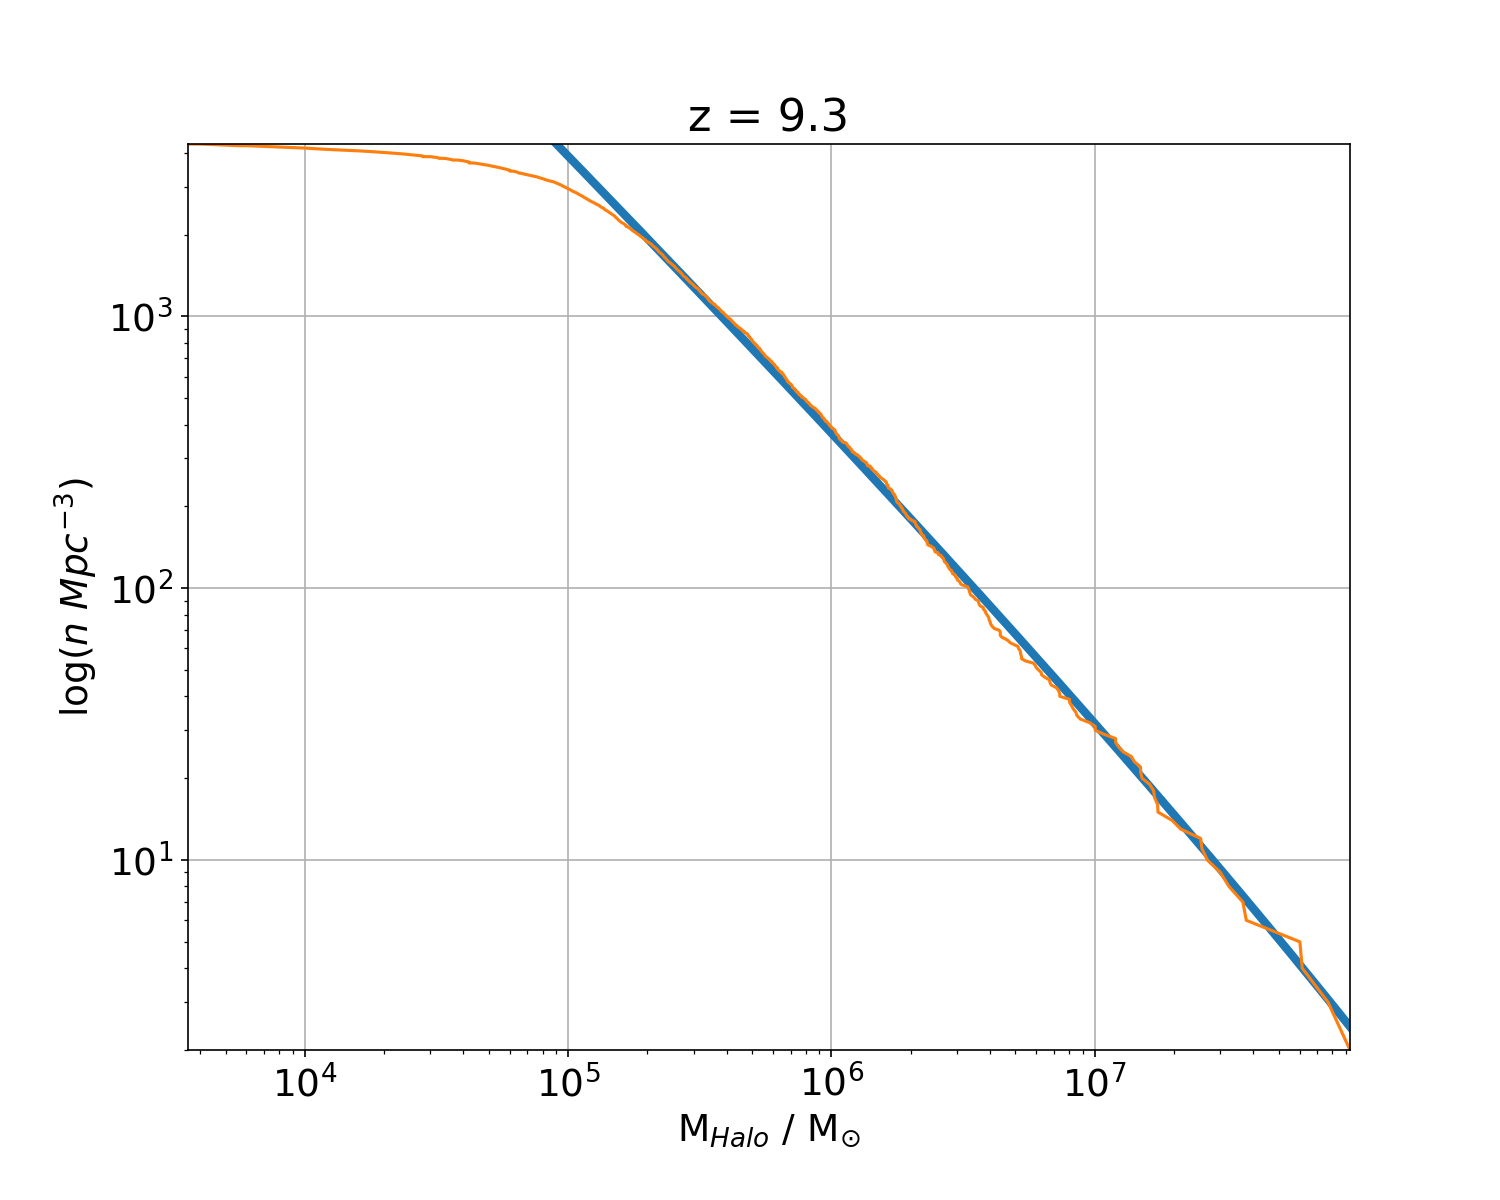
\includegraphics[width=\columnwidth]{images/hmf.png}
    \caption{Halo mass function of the last output of the simulation at $z$ = 9.3. The thick line is the analytic Sheth-Tormen mass function. The distribution of halo masses matches well with Sheth-Tormen until about 10$^{5}$ M$_{\odot}$.}
    \label{fig:hmf}
\end{figure}

\begin{figure}
	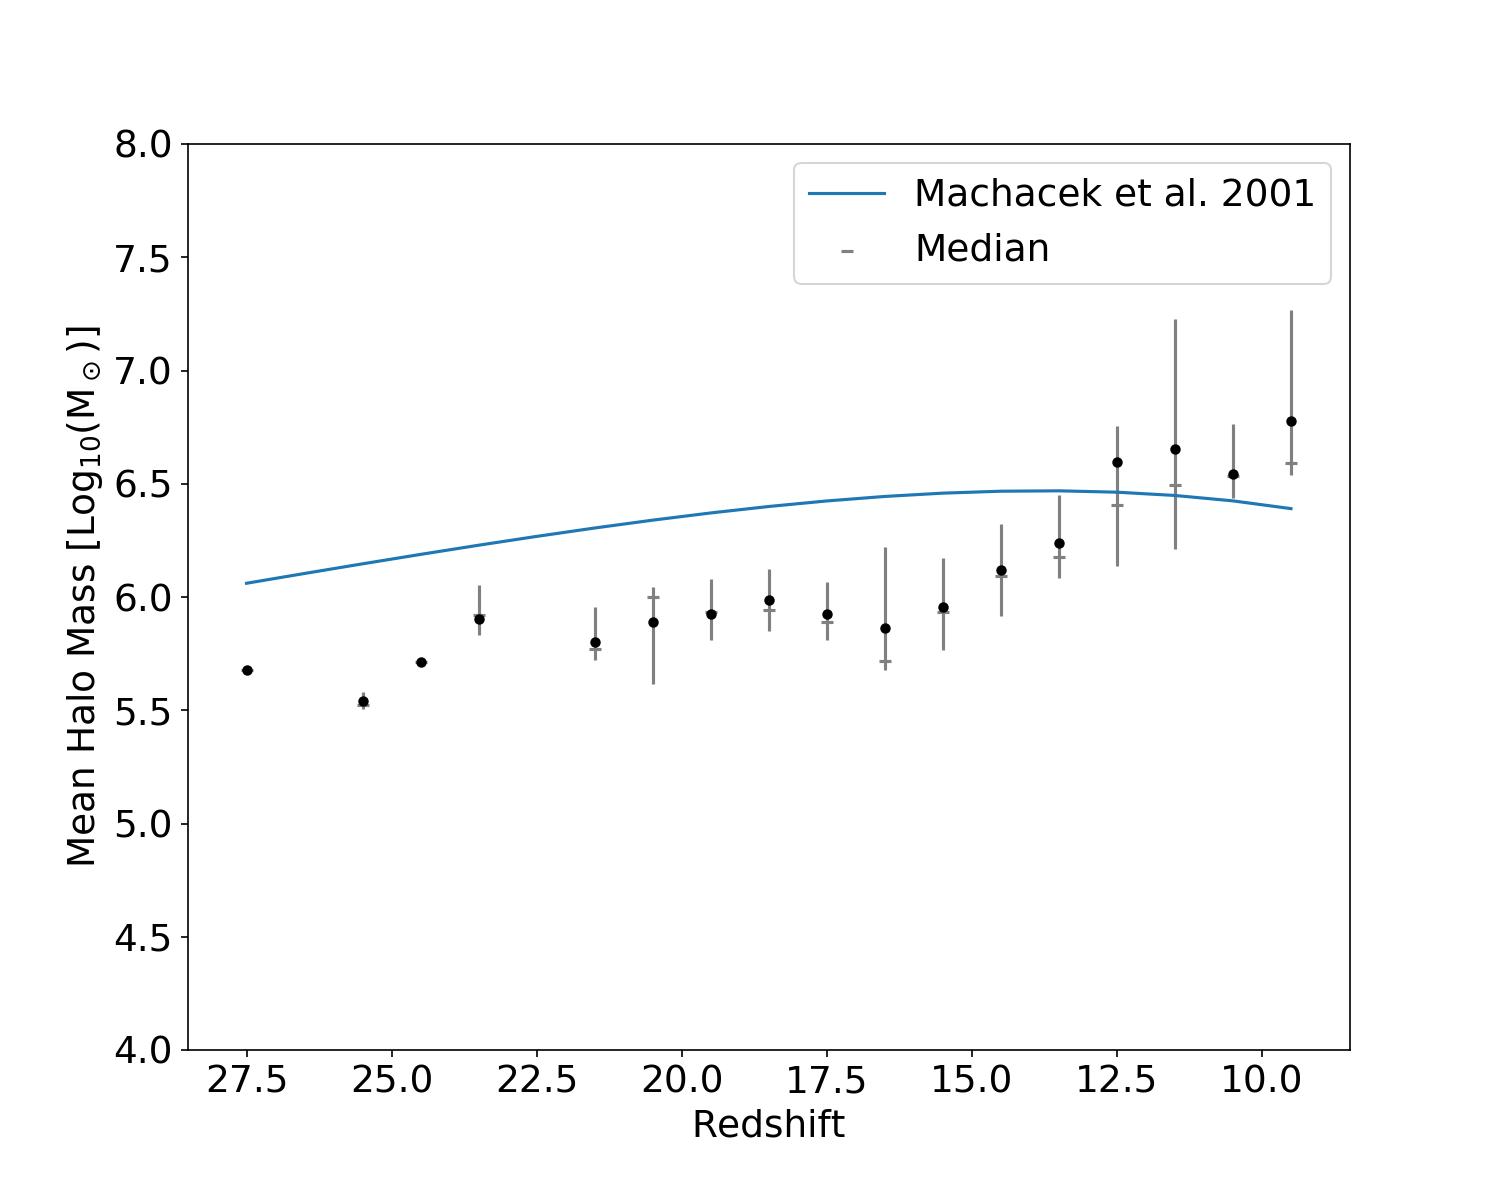
\includegraphics[width=\columnwidth]{images/mean_mass_errorb_fix.png}
    \caption{For halos hosting new Pop III stars, the mean halo mass is plotted versus redshift, in bins of $\Delta z$ = 1. The Machacek et al. minimum mass threshold is plotted for the constant LW background given in Eq. \ref{LWbg}. The mean halo masses fall below the relation until a redshift of 12.5, at which point the mean halo masses rise above the relation.}
    \label{fig:mean_mass}
\end{figure}

\begin{figure}
	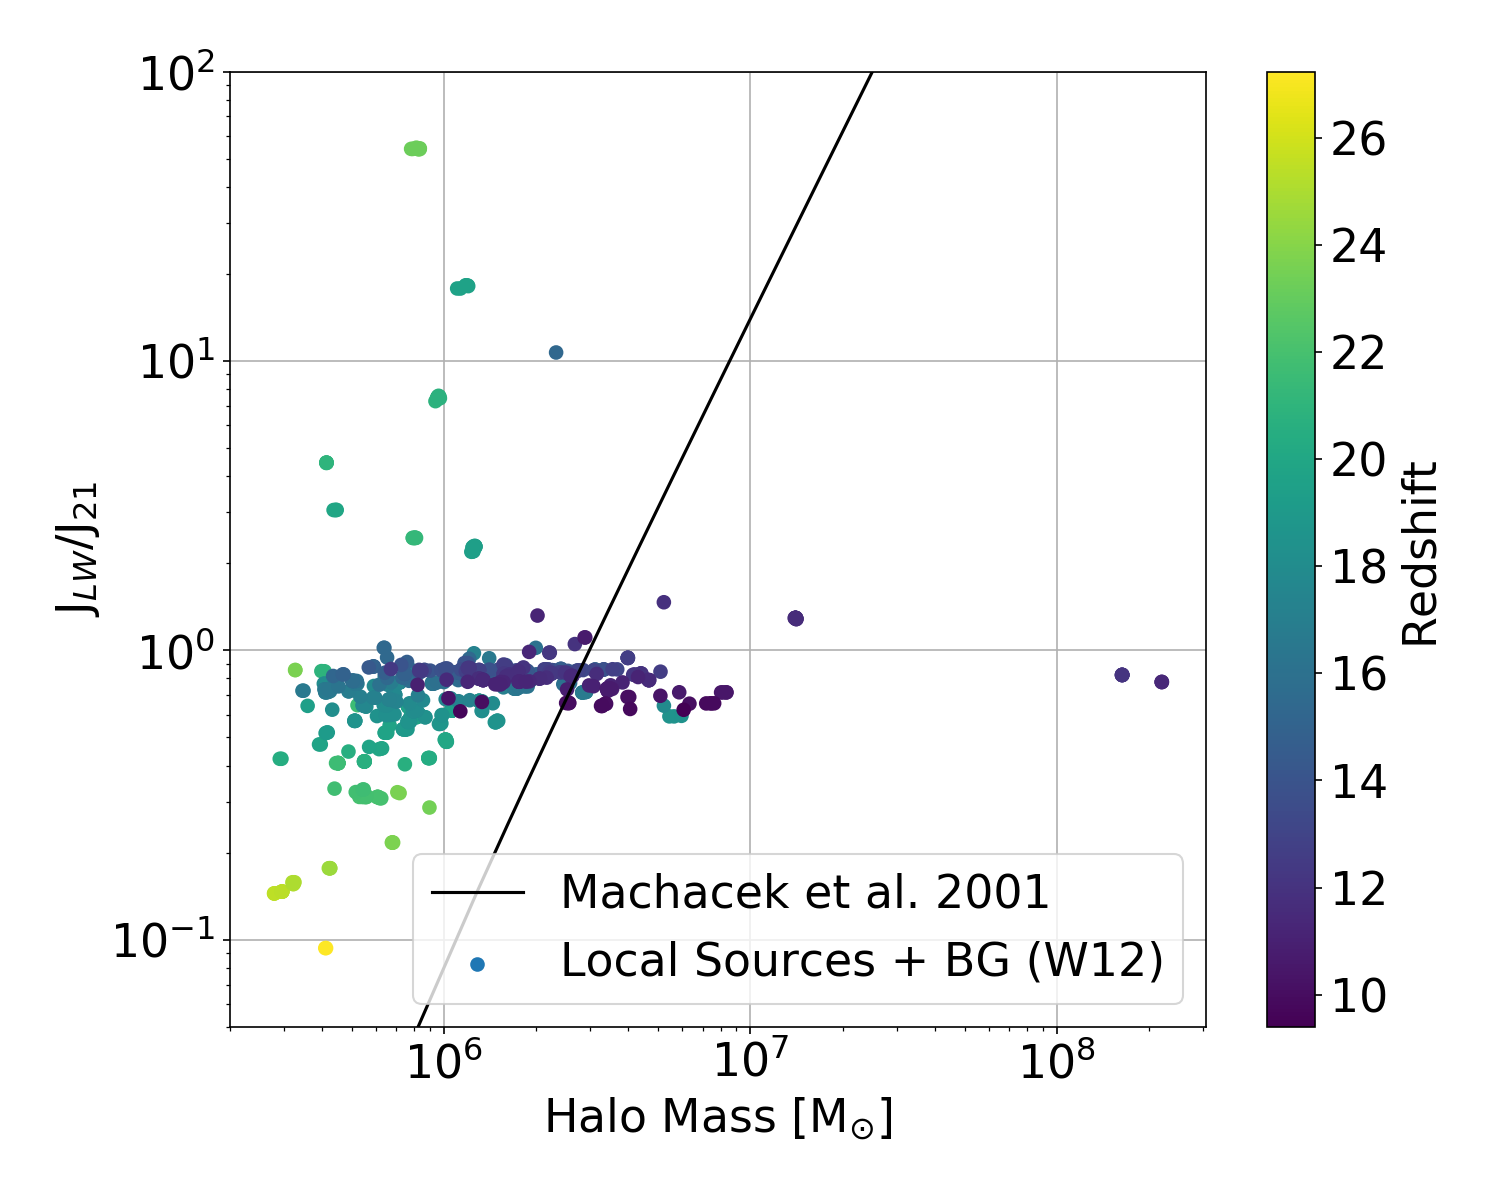
\includegraphics[width=\columnwidth]{images/jlw_mass_machacek_total.png}
    \caption{The average LW background for host halos of new Pop III stars is plotted versus the host halo mass, colored by redshift. The Machacek et al. relation is plotted given the background LW in Eq. \ref{LWbg}. Almost all halos fall below the relation, across a range of redshifts. A few halos (or possibly a single halo) allow Pop III stars to form at a low halo mass in a very high LW background. There are a few halos that have Pop III stars forming at later times and at high halo masses.}
    \label{fig:jlw_mass_machacek}{}
\end{figure}

\begin{figure}
	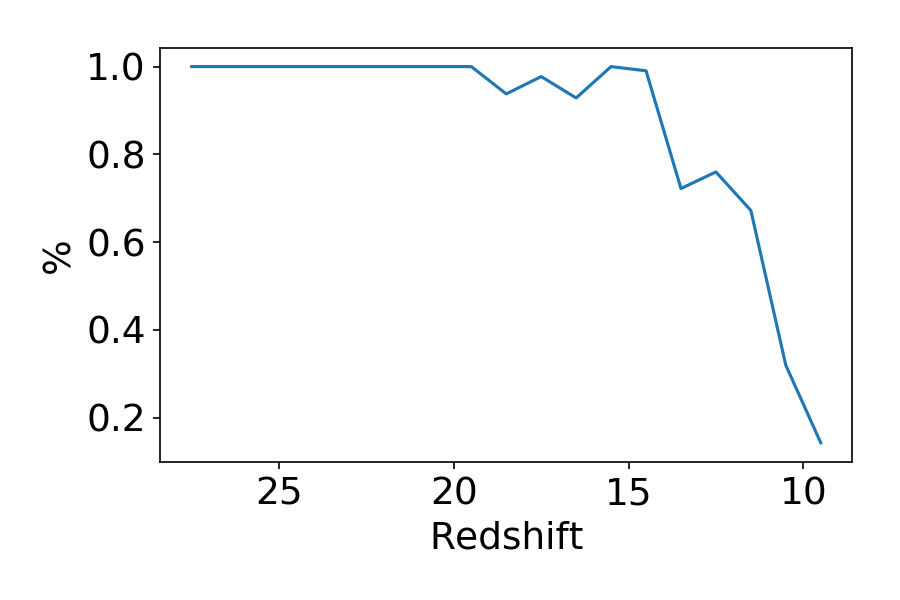
\includegraphics[width=\columnwidth]{images/percent_below_dz1.png}
    \caption{The percentage of halos that form Pop III stars below the minimum mass threshold from \citet{Machacek01}, in bins of $\Delta z$ = 1. As seen in \ref{fig:jlw_mass_machacek}, almost all halos form below the mass threshold.}
    \label{fig:percent_below_dz1}
\end{figure}

\begin{figure}
	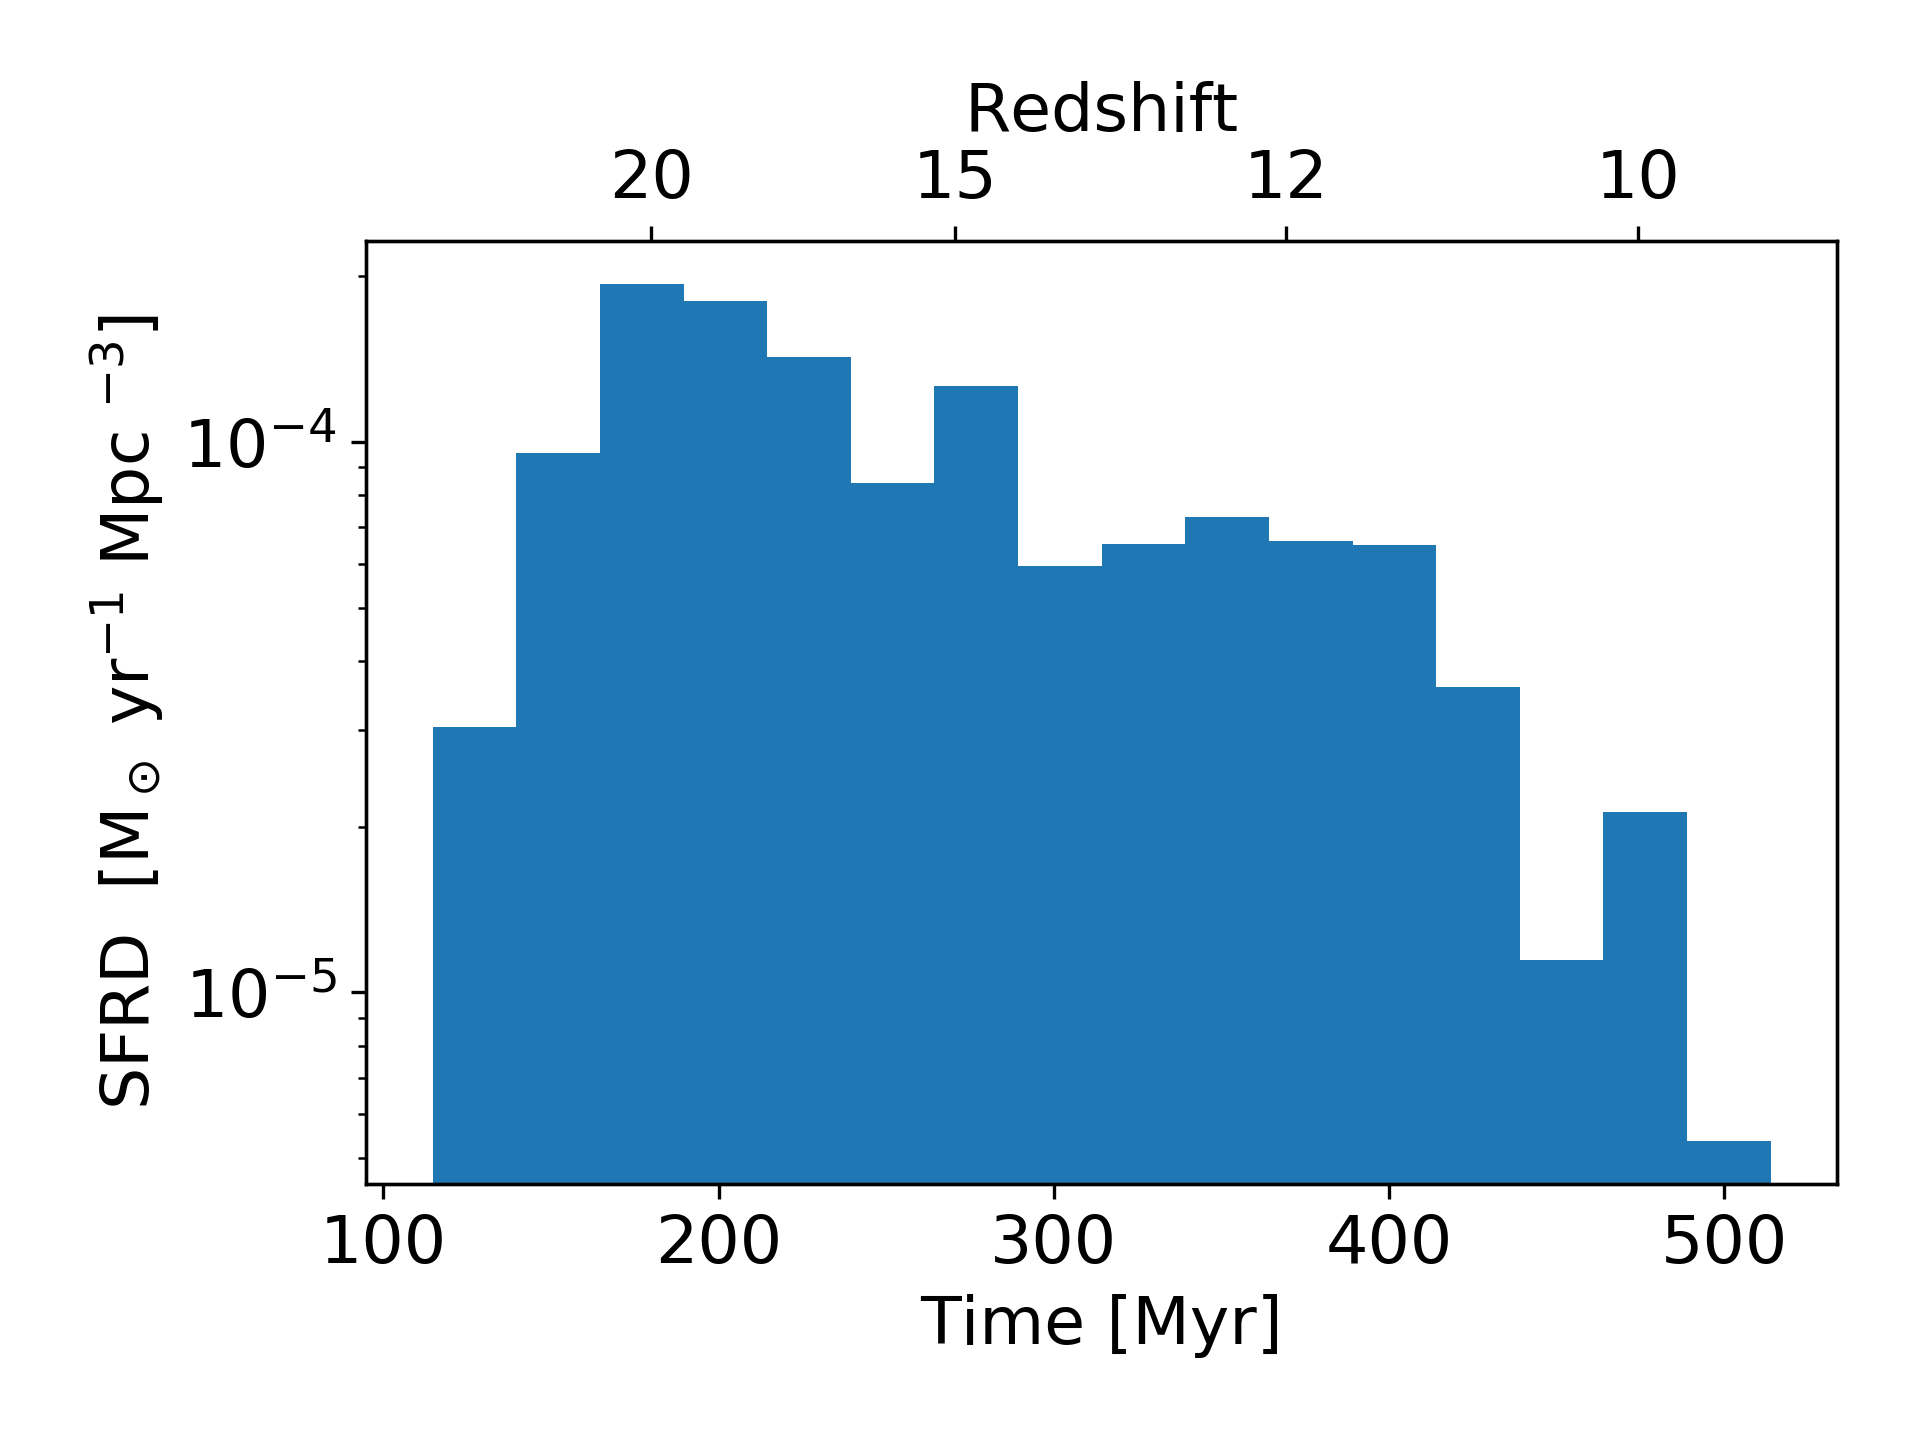
\includegraphics[width=\columnwidth]{images/pop3_SFR_bar.png}
    \caption{The star formation rate density of Pop III stars. It peaks at a redshift of 20, and slowly falls off.}
    \label{fig:pop3_SFR_bar}
\end{figure}

\begin{figure}
	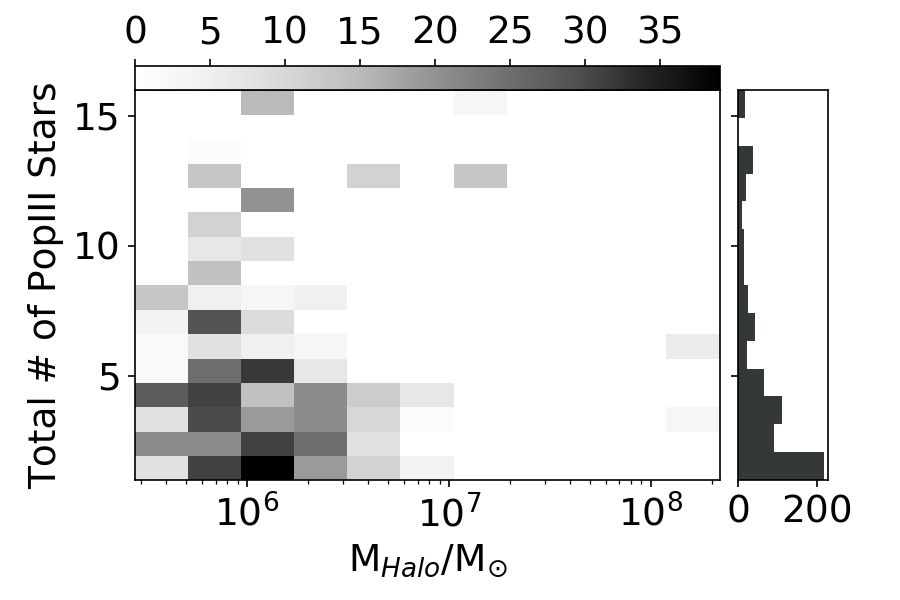
\includegraphics[width=\columnwidth]{images/totnump3_halomass_sidehist.png}
    \caption{Total number of Pop III stars in halos hosting new Pop III stars versus halo mass. A median number of four Pop III stars form in a single halo, with some forming as many as 16 Pop III stars.}
    \label{fig:totnump3_halomass_sidehist}
\end{figure}

\begin{figure}
	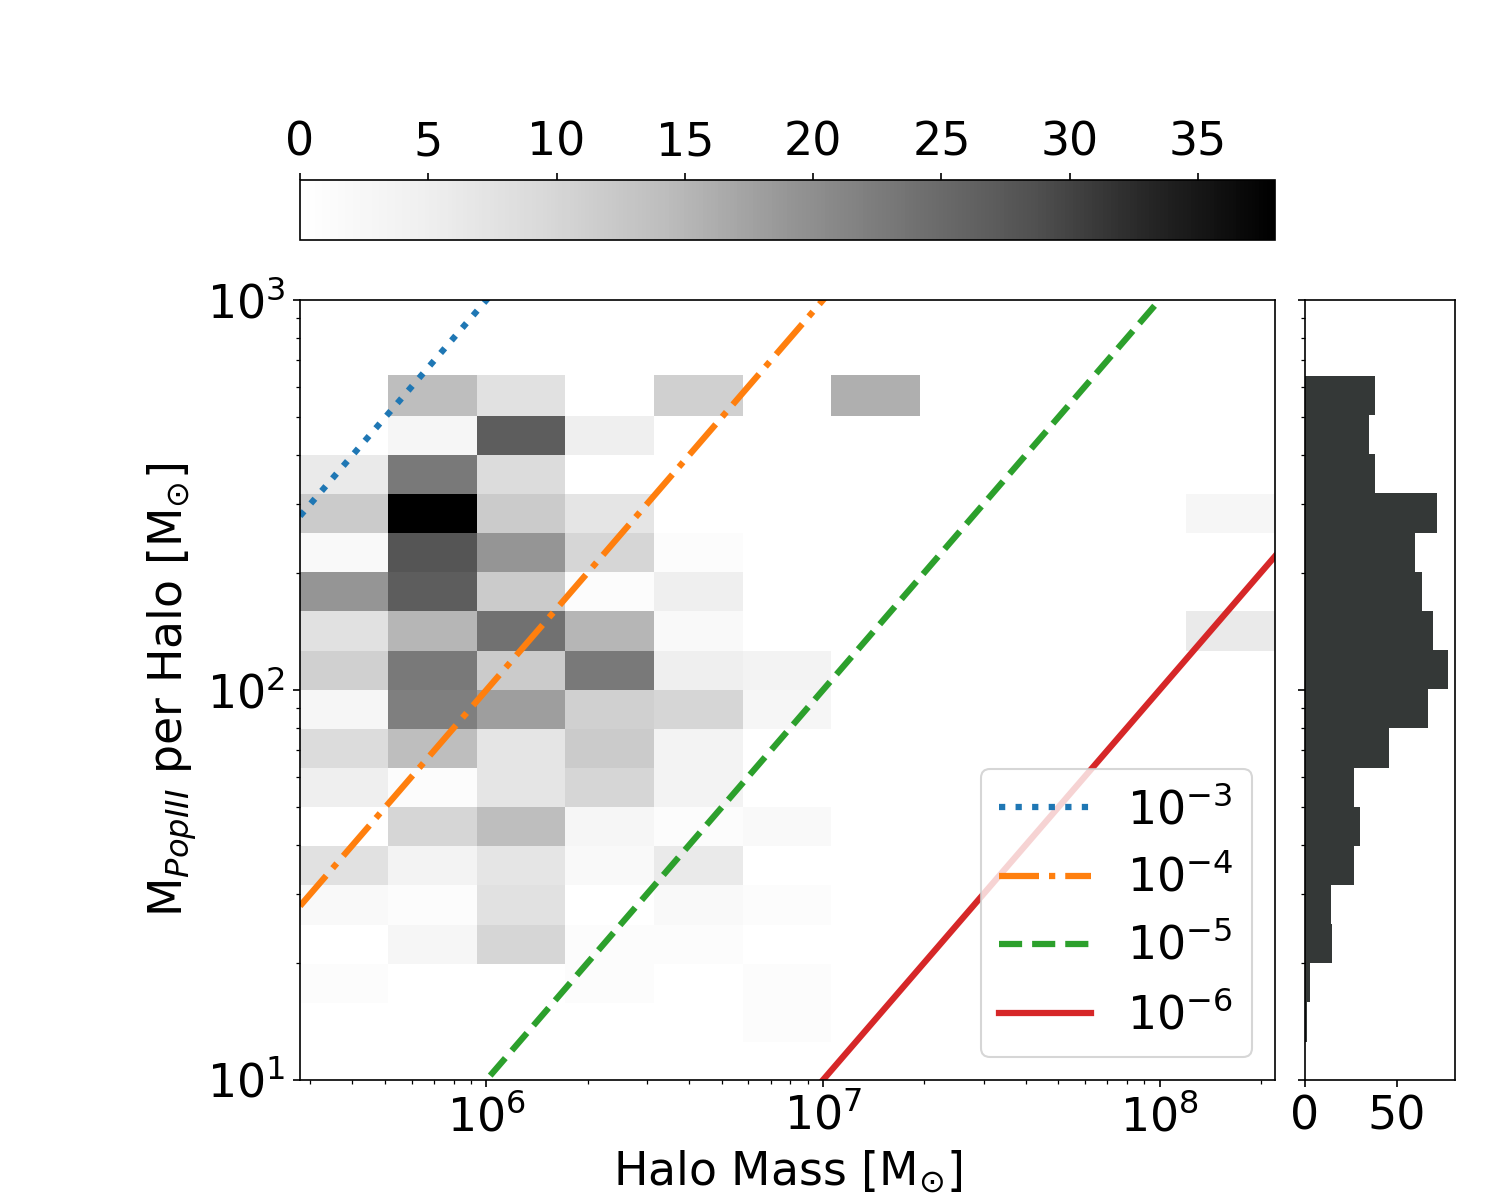
\includegraphics[width=\columnwidth]{images/totp3mass_halomass_sidehist.png}
    \caption{Total mass of Pop III stars in halos hosting new Pop III stars versus halo mass. Lines of constant star formation efficiencies are overplotted. Most halos form Pop III stars at efficiencies between 10$^{-3}$ and 10$^{-4}$.}
    \label{fig:totp3mass_halomass_sidehist}
\end{figure}



%====================================================================
\subsection{Population III host halo masses}
%====================================================================

%====================================================================
\subsection{Multiple stellar systems}
%====================================================================

%====================================================================
\subsection{Population III stars in atomic cooling halos}
%====================================================================

%====================================================================
\section{Discussion}
%====================================================================

%====================================================================
\subsection{Variations in the halo masses at collapse}
%====================================================================

\li Halos can form metal-free stars again if their progenitors had
only formed stars that did not go supernova

\li Dynamical heating \citep{Yoshida03}

\li Temporal fluctuations in the local Lyman-Werner radiation

%====================================================================
\subsection{Comparison to previous work}
%====================================================================

\li Semi-analytic papers: \citep{Tegmark97, Trenti09, Visbal18,
  Mebane18, Griffen18}

\li Simulation papers: \citep{Machacek01, Yoshida03, Wise07_UVB,
  OShea08, Muratov13}

\li We don't have to compare with all of the semi-analytic papers, but
it will be good to compare with all of the simulation papers.

%====================================================================
\subsection{Caveats}
%====================================================================

\li Optically-thin Lyman-Werner radiation field from point sources \citep{Schauer17}

\li No streaming velocities that suppresses star formation at very
high ($z \ga 20$) redshifts \citep{Tselia11, Greif11_Delay, Naoz12, OLeary12}

\li Uncertainties from the assumed Pop III initial mass function 

%====================================================================
\section{Conclusions}
%====================================================================

%====================================================================
\section*{Acknowledgements}
%====================================================================

JHW is supported by National Science Foundation grants AST-1614333 and
OAC-1835213, NASA grant NNX17AG23G, and Hubble theory grant
HST-AR-14326.  We thank the support staff at Georgia Tech's PACE,
where we ran this simulation.  The freely available plotting library
{\sc matplotlib} \citep{matplotlib} was used to construct numerous
plots within this paper. Computations and analysis described in this
work were performed using the publicly-available \enzo{} and \yt{}
codes, which is the product of a collaborative effort of many
independent scientists from numerous institutions around the world.

%%%%%%%%%%%%%%%%%%%%%%%%%%%%%%%%%%%%%%%%%%%%%%%%%%

%%%%%%%%%%%%%%%%%%%% REFERENCES %%%%%%%%%%%%%%%%%%

% The best way to enter references is to use BibTeX:

\bibliographystyle{mnras}
\bibliography{jwise} % if your bibtex file is called example.bib


% Alternatively you could enter them by hand, like this:
% This method is tedious and prone to error if you have lots of references
%\begin{thebibliography}{99}
%\end{thebibliography}

%%%%%%%%%%%%%%%%%%%%%%%%%%%%%%%%%%%%%%%%%%%%%%%%%%

%%%%%%%%%%%%%%%%% APPENDICES %%%%%%%%%%%%%%%%%%%%%

\appendix

%%%%%%%%%%%%%%%%%%%%%%%%%%%%%%%%%%%%%%%%%%%%%%%%%%


% Don't change these lines
\bsp	% typesetting comment
\label{lastpage}
\end{document}

% End of mnras_template.tex